\documentclass[11pt]{article}
% ---------------------------------------------------------------------------
% Reading the Book -- subscription signals and the IPO pop. pdfLaTeX + BibTeX (Overleaf default).
% tables/ and figures/ are generated by make_paper3.py from ../data/signals.json and ../data/pm.json.
% ---------------------------------------------------------------------------
\usepackage[T1]{fontenc}
\usepackage[utf8]{inputenc}
\usepackage{mathpazo}
\usepackage[scaled=0.92]{helvet}
\usepackage{microtype}
\usepackage[a4paper,margin=2.4cm]{geometry}
\usepackage{amsmath,amssymb}
\usepackage{booktabs,threeparttable,array,tabularx,longtable}
\usepackage{graphicx}
\usepackage[font=small,labelfont=bf,labelsep=period,skip=4pt]{caption}
\usepackage{xcolor}
\usepackage{enumitem}
\usepackage[round,authoryear]{natbib}
\usepackage{fancyhdr}
\usepackage{titlesec}
\usepackage[colorlinks=true,linkcolor=accent,citecolor=accent,urlcolor=accent]{hyperref}

\definecolor{accent}{HTML}{1C5CAB}
\definecolor{muted}{HTML}{52514E}
\titleformat{\section}{\normalfont\large\bfseries\color{accent}}{\thesection}{0.8em}{}
\titleformat{\subsection}{\normalfont\normalsize\bfseries}{\thesubsection}{0.8em}{}
\setlength{\parskip}{0.35em}
\setlist{itemsep=0.2em,topsep=0.3em}
\renewcommand{\arraystretch}{1.12}
\newcolumntype{Y}{>{\raggedright\arraybackslash}X}
\pagestyle{fancy}\fancyhf{}
\fancyhead[L]{\small\color{muted}Sympathy or substitution: related stocks around large IPOs}
\fancyhead[R]{\small\color{muted}15 November 2026}
\fancyfoot[C]{\small\thepage}
\renewcommand{\headrulewidth}{0.4pt}

\title{\vspace{-1.2em}\textbf{Sympathy or Substitution?}\\[0.3em]
\large How Related Stocks Trade Around Large IPOs, Intraday and Close to Close,\\ and What It Implies for Anthropic's Peers}
\author{CrossAssetMacro Research}
\date{15 November 2026\\[0.2em]\small Daily data to 13 November 2026; hourly data since November 2024}

\begin{document}
\maketitle
\thispagestyle{fancy}

\begin{abstract}
\noindent When a large IPO trades up, do its listed peers trade up with it? The question matters for Anthropic, whose debut on 19 November could plausibly move Nebius, CoreWeave, Nvidia or its shareholders Amazon and Google. We test it on 43 large US IPOs since 2020 and 88 listed comparables, using daily abnormal returns against Nasdaq-100 and, for the 14 IPOs since 2025, 60-minute bars. \textbf{There is no beta trade from the IPO to its peers.} On the first day the peer basket's abnormal return averages $-0.3\%$ and is unrelated to the size of the pop. Intraday, during the first five sessions, the peers' hourly beta to the new stock is 0.02--0.03, about a fifth of its level once the stock is seasoned; in the debut week the IPO trades on its own flows. Daily correlation with peers starts at 0.32 and rises to 0.48 after three months. Neither leads the other, hourly or daily. The one repeatable pattern runs the other way: \textbf{substitution}. When the IPO is a scarce asset previously reachable only through listed proxies, the proxies fall as the real thing lists: SpaceX's proxies fell 13--26\% on its first day (Destiny Tech100 $-26\%$, Rocket Lab $-13\%$, AST SpaceMobile $-17\%$), and Circle's peers had their worst first-print-to-close move in the sample ($z=-4.5$). Over the following quarter peers lag Nasdaq-100 by 9\% on average and fade together with the IPO ($\rho=0.46$), but the lag is concentrated in 2021 and not distinguishable from these stocks' behaviour on random dates. Into Anthropic's IPO, AI infrastructure has already de-rated: since 30 September Nebius is down 51\%, CoreWeave 39\% and Nvidia 29\% against $-8\%$ for Nasdaq-100, while Amazon is up 7\%; the 20-day abnormal returns of Nebius and Nvidia are in the bottom 7\% of what cohort peers did before their IPOs. For the debut itself, the cohort's betas imply that a 30\% Anthropic pop would lift AI peers by under 1\% intraday and about 2.6\% on the day, before any substitution flow.
\end{abstract}

\section*{Key findings}
\begin{enumerate}[leftmargin=1.4em]
\item \textbf{No sympathy on the day.} Peer-basket abnormal return on the first trading day: mean $-0.3\%$, 95\% CI $[-1.4\%, +0.7\%]$. Correlation with the IPO's pop: 0.19 ($p=0.23$). Hot deals: $+0.6\%$ (Table~\ref{tab:b1}--\ref{tab:b3}).
\item \textbf{No intraday beta in the debut week.} Peers' hourly beta on the IPO's excess return is 0.024 in days 1--5 against 0.129 from day 6 ($t=-5.4$ for the difference). Hourly correlation 0.14, rising to 0.33 by days 22--63 (Table~\ref{tab:b5}).
\item \textbf{No lead--lag.} Neither the IPO's return this hour (or day) predicts its peers' next hour (or day), nor the reverse.
\item \textbf{New issues are their own factor at first.} Daily correlation with peers 0.32 in the first month vs 0.48 after three months ($p=0.001$); IPO volatility twice the peer basket's (Table~\ref{tab:b4}).
\item \textbf{The exception is substitution.} When an IPO lists a scarce asset, the listed proxies sell off: SpaceX proxies $-13\%$ to $-26\%$ on day 0 and further over the month; Circle's peers fell from its first print to the close (Tables~\ref{tab:b6}, \ref{tab:b8}).
\item \textbf{Peers fade with the IPO, not because of it.} Peer and IPO 63-day returns co-move ($\rho=0.46$); peers lag by $-9\%$ on average, but that is 2021-driven and at the 24th percentile of a placebo distribution.
\item \textbf{Anthropic's peers have pre-sold.} AI infrastructure has de-rated into the deal (Nebius, Nvidia in the bottom 7\% of cohort pre-IPO peers on 20-day abnormal returns); Amazon, a shareholder, has outperformed (88th percentile) while Google, also a shareholder, has lagged (Table~\ref{tab:b7}).
\end{enumerate}

\section{Question and design}
A new listing can affect related stocks through three channels. \textit{Sympathy}: the IPO's price reveals information about the value of the sector, so a big pop re-rates peers up \citep{slovin1994}. \textit{Substitution}: investors who held peers as the closest available exposure switch into the new stock, selling the peers to fund it; if the IPO is a better or purer exposure, the proxies' scarcity premium disappears \citep{braun2016}. \textit{Competition}: a newly funded rival takes market share and the peers underperform over months \citep{hsu2010}. The trader's version of the question is simpler: if Anthropic trades up, does Nebius trade up with it, and should one trade the beta?

\paragraph{Sample.} The 43 large US IPOs since September 2020 used in the companion papers \citep{frenzyfade2026}. For each we pick two to four listed comparables that were trading at least six months before the IPO (88 distinct stocks), plus listed stakeholders where they exist: Amazon and Ford for Rivian, Shopify for Klaviyo, Nvidia for CoreWeave, Coinbase for Circle, and Google and the Destiny Tech100 fund (DXYZ) for SpaceX. The peer map is in Appendix~\ref{app:map}. Daily prices since 2019 and 60-minute bars since November 2024 come from Yahoo Finance; hourly data cover the 14 IPOs since January 2025.

\paragraph{Measures.} Abnormal returns use a market model on QQQ estimated over days $-260$ to $-21$. We average across peers to one basket per IPO so that every IPO has equal weight. Hourly returns are taken net of QQQ with overnight gaps excluded. Inference uses $t$-tests and bootstrap intervals across IPO baskets, Wilcoxon and Mann--Whitney tests, panel regressions with errors clustered by IPO, and a placebo that re-runs the event study on the same peers at 400 sets of random dates.

\section{Close to close: no sympathy, a slow fade}
Figure~\ref{fig:path} and Table~\ref{tab:b1} give the average peer path. Peers do not run up into the IPO (days $-10$ to $-1$: $-1.1\%$, $p=0.39$), do not move on the day ($-0.3\%$) and are flat for the following week ($-0.7\%$). They then drift lower: $-3.0\%$ by day 21 ($p=0.055$) and $-9.4\%$ by day 63 ($p=0.013$, 37\% of baskets positive). Listed stakeholders, only five cases, look similar on the day ($-2.9\%$, not significant).

\begin{figure}[!htbp]\centering
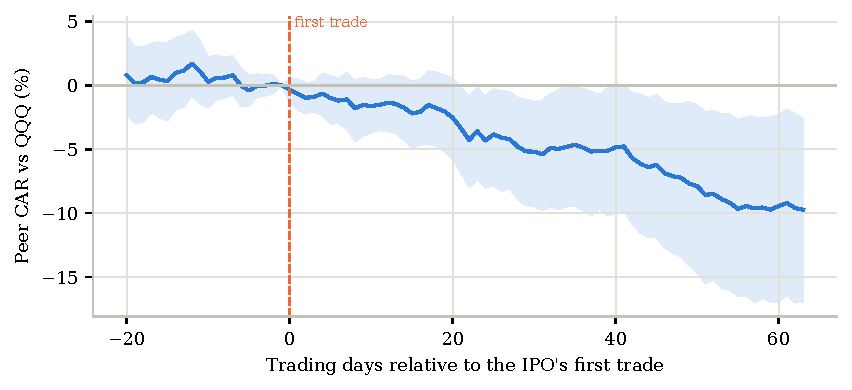
\includegraphics[width=0.9\linewidth]{figures/g1_path}
\caption{Mean cumulative abnormal return of the peer basket against QQQ, rebased to zero at the close before the IPO; shaded area = 95\% bootstrap interval, 43 IPOs. Peers are flat through the debut and drift lower over the following quarter.}\label{fig:path}
\end{figure}

\begin{table}[!htbp]\centering\footnotesize
\caption{How related stocks trade around an IPO: abnormal returns against Nasdaq-100}\label{tab:b1}
\resizebox{\linewidth}{!}{
\begin{threeparttable}
\begin{tabular}{lrrrrrr}
\toprule
Window & $n$ & Mean & Median & 95\% CI & $p$ & Share $>0$ \\
\midrule
\multicolumn{7}{l}{\textit{Comparable listed companies (equal-weight basket per IPO)}} \\
\quad Days $-20$ to $-1$ & 43 & $-$0.7 & $-$2.1 & [$-$3.9, +2.7] & 0.69 & 37\% \\
\quad Days $-10$ to $-1$ (roadshow) & 43 & $-$1.1 & $-$0.9 & [$-$3.5, +1.3] & 0.39 & 37\% \\
\quad Days $-5$ to $-1$ & 43 & 0.0 & $-$0.7 & [$-$1.6, +1.6] & 0.99 & 40\% \\
\quad Day 0 (first trade) & 43 & $-$0.3 & $-$0.1 & [$-$1.4, +0.7] & 0.53 & 44\% \\
\quad Day 0, open to close & 43 & $-$0.2 & +0.1 & [$-$1.2, +0.6] & 0.71 & 53\% \\
\quad Days 1 to 5 & 43 & $-$0.7 & $-$0.3 & [$-$2.0, +0.7] & 0.37 & 47\% \\
\quad Days 1 to 21 & 43 & $-$3.0 & $-$1.2 & [$-$6.1, $-$0.1] & 0.055 & 42\% \\
\quad Days 1 to 63 & 43 & $-$9.4 & $-$4.6 & [$-$16.5, $-$2.2] & 0.013 & 37\% \\
\multicolumn{7}{l}{\textit{Listed stakeholders (Amazon, Ford, Shopify, Nvidia, Coinbase, Google, DXYZ)}} \\
\quad Days $-10$ to $-1$ (roadshow) & 5 & $-$6.3 & $-$10.0 & [$-$13.5, +3.7] & 0.26 & 20\% \\
\quad Day 0 (first trade) & 5 & $-$2.9 & $-$2.3 & [$-$8.6, +1.4] & 0.37 & 20\% \\
\quad Days 1 to 5 & 5 & $-$2.1 & $-$4.3 & [$-$6.7, +3.5] & 0.50 & 40\% \\
\quad Days 1 to 21 & 5 & +2.7 & $-$4.4 & [$-$6.7, +16.7] & 0.73 & 40\% \\
\midrule
\multicolumn{7}{l}{Placebo percentile of the actual mean (400 random event dates): day 0 31\%, days 1--21 31\%, days 1--63 24\%} \\
\bottomrule
\end{tabular}
\begin{tablenotes}[flushleft]\footnotesize
\item \textit{Notes:} Percent. Abnormal return = stock return minus a market model on QQQ estimated over days $-260$ to $-21$. 102 peer--IPO pairs (88 distinct stocks) across 43 IPOs; one basket per IPO. CI by bootstrap, $p$ from a $t$-test across IPO baskets. Placebo: the same peers on random dates within $\pm$1 year, using full-sample market models.
\end{tablenotes}
\end{threeparttable}
}
\end{table}


The 63-day drift is less solid than its $p$-value suggests. It comes mostly from 2021, when nine IPOs listed near the peak of growth-stock valuations and their peers fell 23\% against QQQ in the next quarter. Excluding 2021, the drift is $-5.8\%$ ($p=0.16$). And the placebo, which applies the same calculation to the same peers on random dates, puts the actual 63-day number at only the 24th percentile: these are high-beta growth stocks whose returns against QQQ swing widely whatever the date. We read it as weak evidence for the competitive effect of \citet{hsu2010}, not as a tradable pattern.

\begin{table}[!htbp]\centering\footnotesize
\caption{Peer abnormal returns by IPO demand and by vintage}\label{tab:b2}
\resizebox{\linewidth}{!}{
\begin{threeparttable}
\begin{tabular}{lrrrrrr}
\toprule
Group & $n$ & Days $-10$ to $-1$ & Day 0 & Days 1--5 & Days 1--21 & Days 1--63 \\
\midrule
Hot & 20 & +1.6 & +0.6 & 0.0 & 0.0 & $-$6.8 \\
Not hot & 23 & $-$3.5 & $-$1.1 & $-$1.3 & $-$5.6 & $-$11.7 \\
Pop $>$ 30\% & 17 & $-$0.3 & +0.6 & $-$1.1 & +0.9 & $-$4.6 \\
Pop $\le$ 30\% & 26 & $-$1.6 & $-$0.9 & $-$0.4 & $-$5.6 & $-$12.5 \\
Mann--Whitney $p$, hot vs not & & 0.10 & 0.053 & 0.65 & 0.15 & 0.60 \\
\midrule
2021 IPOs only & 9 & -- & +1.0 & -- & $-$6.3 ($p$=0.042) & $-$23.0 ($p$=0.010) \\
Excluding 2021 & 34 & -- & $-$0.7 & -- & $-$2.1 ($p$=0.24) & $-$5.8 ($p$=0.16) \\
IPOs since 2023 & 30 & -- & $-$0.9 & -- & $-$3.4 ($p$=0.069) & $-$9.4 ($p$=0.029) \\
\bottomrule
\end{tabular}
\begin{tablenotes}[flushleft]\footnotesize
\item \textit{Notes:} Mean peer-basket abnormal return, percent. Hot = range raised and priced above it.
\end{tablenotes}
\end{threeparttable}
}
\end{table}


Demand does not change the picture much (Table~\ref{tab:b2}). Peers of hot deals did slightly better on the day ($+0.6\%$ vs $-1.1\%$, $p=0.053$) and lagged less afterwards, consistent with a hot book reflecting a strong sector rather than causing one. Table~\ref{tab:b3} confirms there is no dose--response: the size of the pop is unrelated to the peers' move on the day ($\rho=0.19$) or over the next quarter ($\rho=-0.01$). The only significant link is that IPO and peers fade \emph{together} over 63 days ($\rho=0.46$, $p=0.002$): when the theme unwinds, the new issue and its peers go down at the same time.

\begin{table}[!htbp]\centering\footnotesize
\caption{Does a bigger debut move peers more? Cross-section of 43 IPOs}\label{tab:b3}

\begin{threeparttable}
\begin{tabular}{lrrr}
\toprule
Pair & Spearman $\rho$ & $p$ & $n$ \\
\midrule
Peers day 0 vs IPO opening pop & 0.21 & 0.17 & 43 \\
Peers day 0 vs IPO first-day return & 0.19 & 0.23 & 43 \\
Peers day 0 vs IPO open-to-close & $-$0.02 & 0.91 & 43 \\
Peers days 1--5 vs IPO days 1--5 & 0.21 & 0.17 & 43 \\
Peers days 1--21 vs IPO days 1--21 & 0.15 & 0.34 & 43 \\
Peers days 1--63 vs IPO days 1--63 & 0.46 & 0.002 & 43 \\
Peers roadshow run-up vs IPO first-day return & $-$0.04 & 0.81 & 43 \\
Peers days 1--63 vs IPO first-day return & $-$0.01 & 0.92 & 43 \\
\bottomrule
\end{tabular}
\begin{tablenotes}[flushleft]\footnotesize
\item \textit{Notes:} Peer returns are basket abnormal returns; IPO returns are raw. Only the 63-day co-movement is significant: IPO and peers fade together over a quarter, but the size of the debut does not move peers on the day.
\end{tablenotes}
\end{threeparttable}

\end{table}


\section{Co-movement: the new issue is its own factor}
Table~\ref{tab:b4} measures how tightly the IPO trades with its peers as it seasons. In the first month the median daily correlation with the peer basket is 0.32; after three months it is 0.48 (Wilcoxon $p=0.001$). The IPO's volatility is twice the basket's at first and 1.5 times later. Its loading on the theme, after removing the market, is about 0.5 throughout, so the low early correlation reflects extra idiosyncratic noise from allocation flipping, unfilled demand and absent short supply, not a different exposure. This is the pattern \citet{barberis2005} and \citet{greenwood2008} describe for index inclusion: correlation with a group rises once a stock is held and traded by the same investors as the group.

\begin{table}[!htbp]\centering\footnotesize
\caption{Daily co-movement: new issues trade on their own at first}\label{tab:b4}
\resizebox{\linewidth}{!}{
\begin{threeparttable}
\begin{tabular}{lrrr}
\toprule
Median across IPOs & Days 1--21 & Days 22--63 & Days 64--190 \\
\midrule
Correlation, IPO vs peer basket & 0.32 & 0.39 & 0.48 \\
Beta to QQQ & 1.21 & 1.64 & 1.38 \\
Beta to the theme (peer basket ex-QQQ) & 0.48 & 0.43 & 0.55 \\
Volatility, IPO / peer basket & 1.98 & 1.77 & 1.46 \\
$R^2$ (QQQ + theme) & 0.17 & 0.23 & 0.26 \\
Peer basket beta to QQQ & 1.16 & 1.14 & 1.11 \\
\midrule
Wilcoxon $p$, days 1--21 vs 64--190: correlation 0.001; theme beta 0.53 & & & \\
\midrule
\multicolumn{4}{l}{\textit{Pooled daily panel, days 1--21, excess returns over QQQ, clustered by IPO}} \\
Peers today on IPO today & 0.086 & $t$=4.2 & $n$=903 \\
Peers tomorrow on IPO today & $-$0.011 & $t$=$-$1.0 & \\
IPO tomorrow on peers today & 0.044 & $t$=0.5 & \\
\bottomrule
\end{tabular}
\begin{tablenotes}[flushleft]\footnotesize
\item \textit{Notes:} Daily returns. Theme beta from a regression of the IPO's return on QQQ and on the peer basket orthogonalised to QQQ.
\end{tablenotes}
\end{threeparttable}
}
\end{table}


In a pooled panel of the first 21 days, the peers' excess return rises by 0.086\% for each 1\% of the IPO's excess return on the same day ($t=4.2$). That is a modest common-factor relationship and runs in both directions; neither series predicts the other the next day.

\section{Intraday: is there a beta trade?}
The hourly data answer the trader's question directly. Table~\ref{tab:b5} and Figure~\ref{fig:comove} show that in the first five sessions the peers hardly respond to the IPO's hourly moves: the median beta of peers on the IPO is 0.032 and the median correlation 0.14. Both rise steadily as the stock seasons, to 0.153 and 0.33 by days 22--63. The pooled regression gives the same result with clustered errors: a beta of 0.129 from day 6, minus 0.105 in days 1--5 ($t=-5.4$), so about 0.024 in the debut week. Lead--lag terms are small and insignificant: the IPO's move in one hour does not predict the peers' move in the next.

\begin{table}[!htbp]\centering\footnotesize
\caption{Intraday: is there a beta trade from the IPO to its peers?}\label{tab:b5}
\resizebox{\linewidth}{!}{
\begin{threeparttable}
\begin{tabular}{lrrr}
\toprule
Median across 14 IPOs & Days 1--5 & Days 6--21 & Days 22--63 \\
\midrule
Correlation, IPO vs peers (excess of QQQ) & 0.14 & 0.21 & 0.33 \\
Beta of peers on the IPO & 0.032 & 0.083 & 0.153 \\
Beta of the IPO on peers & 0.63 & 0.45 & 0.62 \\
\midrule
\multicolumn{4}{l}{\textit{Pooled hourly panel, days 1--63, clustered by IPO}} \\
Peers on IPO, same hour, days 6--63 & 0.129 & $t$=7.8 & $n$=6034 \\
\quad extra in days 1--5 & $-$0.105 & $t$=$-$5.4 & \\
Peers next hour on IPO, days 1--5 / later & 0.009 / $-$0.012 & $t$=1.5 / $-$1.3 & \\
IPO next hour on peers, days 1--5 / later & 0.16 / 0.04 & $t$=0.8 / 1.9 & \\
\bottomrule
\end{tabular}
\begin{tablenotes}[flushleft]\footnotesize
\item \textit{Notes:} 60-minute bars, excess of QQQ, overnight gaps excluded. IPOs listed since January 2025: Venture Global, SailPoint, CoreWeave, Hinge Health, Circle, Chime, Figma, Klarna, Figure, Gemini, StubHub, Netskope, Medline, SpaceX.
\end{tablenotes}
\end{threeparttable}
}
\end{table}


\begin{figure}[!htbp]\centering
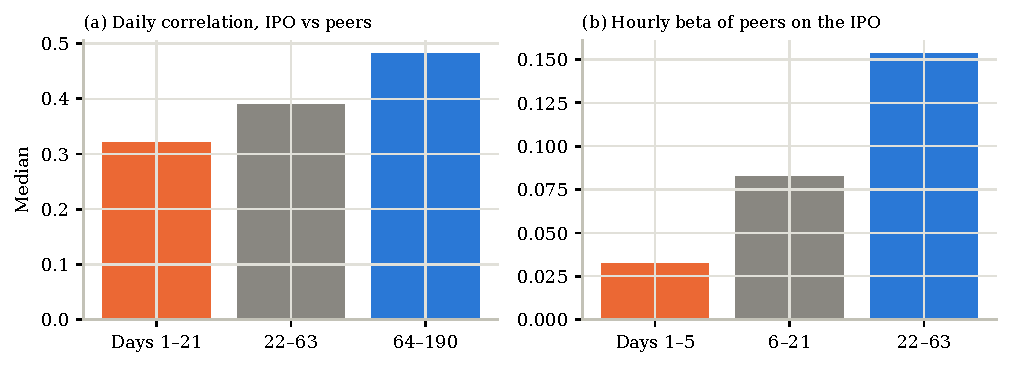
\includegraphics[width=0.9\linewidth]{figures/g2_comove}
\caption{(a) Median daily correlation between the IPO and its peer basket, by window. (b) Median hourly beta of the peer basket on the IPO, excess of QQQ. Debut-week moves are not transmitted to peers.}\label{fig:comove}
\end{figure}

Table~\ref{tab:b6} and Figure~\ref{fig:day1} look at day 1 on the clock: how peers trade from the previous close to the IPO's first print, and from the first print to the close, against the same clock windows on the 20 previous sessions. On average peers do nothing unusual in either window ($-0.6\%$ and $-1.1\%$, neither significant). The distribution has two clear outliers on the downside, Circle ($z=-4.5$) and SpaceX ($z=-5.2$), and the largest positive reading is Netskope ($z=+2.8$), whose cyber-security peers rallied on the day for unrelated reasons.

\begin{table}[!htbp]\centering\scriptsize
\caption{Day 1 on the clock: peers before and after the IPO's first print}\label{tab:b6}
\resizebox{\linewidth}{!}{
\begin{threeparttable}
\begin{tabular}{lllrrrr}
\toprule
IPO & First print (ET) & Peers / stakeholders & Peers: close$\to$first print & Peers: first print$\to$close & IPO open$\to$close & Pop \\
\midrule
Venture Global & 12:30 & LNG, NFE & $-$1.1 ($-$0.7) & $-$0.6 ($-$0.6) & $-$0.4 & $-$4 \\
SailPoint & 13:30 & OKTA, CRWD & +0.7 (0.0) & +1.1 (2.1) & $-$4.3 & $-$4 \\
CoreWeave & 12:30 & NBIS, ORCL, SMCI, NVDA & $-$1.7 ($-$0.5) & $-$0.3 ($-$0.3) & +2.4 & 0 \\
Hinge Health & 12:30 & TDOC, HIMS & $-$2.7 ($-$0.8) & $-$2.1 ($-$1.5) & $-$3.7 & +17 \\
Circle & 12:30 & HOOD, COIN & +2.1 (0.2) & $-$3.3 ($-$4.5) & +19.9 & +168 \\
Chime & 12:30 & SOFI, NU, DAVE & $-$0.9 ($-$0.6) & $-$0.7 ($-$1.2) & $-$14.1 & +37 \\
Figma & 13:30 & ADBE, WIX & $-$1.9 ($-$1.4) & +0.4 (1.2) & +24.4 & +250 \\
Klarna & 10:30 & AFRM, PYPL, SEZL & $-$1.6 ($-$1.0) & $-$0.1 (0.1) & $-$4.5 & +7 \\
Figure & 12:30 & SOFI, UPST, COIN & +1.1 (0.4) & $-$0.3 ($-$0.3) & $-$12.3 & +24 \\
Gemini & 13:30 & COIN, HOOD, CRCL & $-$2.9 ($-$1.1) & $-$0.6 ($-$0.5) & $-$14.0 & +14 \\
StubHub & 11:30 & LYV, SEAT & +3.2 (1.9) & $-$3.3 ($-$1.8) & $-$12.4 & $-$6 \\
Netskope & 11:30 & ZS, CRWD, PANW, NET & +3.0 (2.7) & +1.6 (2.8) & $-$2.0 & +18 \\
Medline & 12:30 & CAH, MCK & +0.7 (0.7) & +1.2 (1.9) & +16.3 & +41 \\
SpaceX & 11:30 & RKLB, ASTS, GOOGL, DXYZ & $-$6.0 ($-$1.2) & $-$7.8 ($-$5.2) & +7.4 & +19 \\
\midrule
Mean & & & $-$0.6 ($p$=0.41) & $-$1.0 ($p$=0.13) & & \\
\bottomrule
\end{tabular}
\begin{tablenotes}[flushleft]\footnotesize
\item \textit{Notes:} Peer basket return minus QQQ over the same clock window, percent; in brackets a $z$-score against the same clock window on the 20 previous sessions. First print = the hourly bar containing the IPO's opening trade.
\end{tablenotes}
\end{threeparttable}
}
\end{table}


\begin{figure}[!htbp]\centering
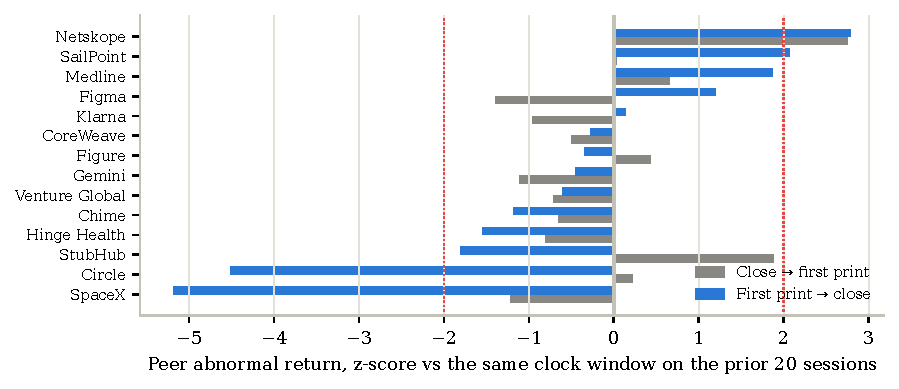
\includegraphics[width=0.85\linewidth]{figures/g3_day1}
\caption{Peer-basket abnormal return on the IPO's first day, before and after the first print, as $z$-scores against the same clock windows on the 20 previous sessions. Dotted lines at $\pm2$. The two large negative readings are the two IPOs of scarce assets with listed proxies.}\label{fig:day1}
\end{figure}

\section{The exception: substitution when a scarce asset lists}
SpaceX and Circle share a feature the rest of the cohort lacks: before listing, investors who wanted exposure had to use proxies. For SpaceX these were the Destiny Tech100 fund, which held SpaceX shares and traded at a large premium to its holdings, and listed space stocks, Rocket Lab and AST SpaceMobile, that traded partly as a SpaceX substitute. For Circle the closest listed exposure was Coinbase, which shares Circle's USDC revenue, and Robinhood. Figure~\ref{fig:cases} shows what happened. DXYZ opened about 20\% lower on SpaceX's first day, before SpaceX had traded, and finished the day down 26\% against QQQ; Rocket Lab and AST fell 13\% and 17\% and kept falling for a month ($-34\%$ and $-24\%$ by day 21). On Circle's first day its peers slid from the first print to the close while Circle nearly tripled.

CoreWeave, the closest precedent for an AI listing, did not show this. Its IPO was cut in size and priced below the range; Nebius fell 5\% on the day but rallied 18\% over the next five sessions as CoreWeave itself rallied (Table~\ref{tab:b8}). AI infrastructure was not a scarce asset in March 2025: listed alternatives were plentiful.

\begin{table}[!htbp]\centering\footnotesize
\caption{The two closest precedents: SpaceX's proxies and CoreWeave's peers}\label{tab:b8}

\begin{threeparttable}
\begin{tabular}{llrrrr}
\toprule
IPO & Stock & Days $-20$ to $-1$ & Day 0 & Days 1--5 & Days 1--21 \\
\midrule
SpaceX (12 Jun 2026) & GOOGL & $-$16.5 & $-$0.3 & $-$6.3 & $-$1.0 \\
SpaceX (12 Jun 2026) & DXYZ & $-$21.7 & $-$26.2 & $-$11.7 & $-$7.8 \\
SpaceX (12 Jun 2026) & RKLB & $-$13.8 & $-$12.7 & $-$9.9 & $-$34.4 \\
SpaceX (12 Jun 2026) & ASTS & +24.7 & $-$17.3 & $-$18.5 & $-$24.3 \\
\midrule
CoreWeave (28 Mar 2025) & NBIS & $-$24.9 & $-$5.1 & +18.3 & $-$15.6 \\
CoreWeave (28 Mar 2025) & ORCL & $-$9.4 & $-$0.6 & +1.4 & $-$2.7 \\
CoreWeave (28 Mar 2025) & SMCI & $-$3.3 & +5.2 & +12.1 & +8.2 \\
CoreWeave (28 Mar 2025) & NVDA & +0.5 & +4.2 & +7.5 & $-$4.5 \\
\bottomrule
\end{tabular}
\begin{tablenotes}[flushleft]\footnotesize
\item \textit{Notes:} Abnormal returns against a QQQ market model, percent. DXYZ (Destiny Tech100) is a listed closed-end fund that held SpaceX shares; Google is a SpaceX shareholder; Rocket Lab and AST SpaceMobile were traded as listed space proxies.
\end{tablenotes}
\end{threeparttable}

\end{table}


\begin{figure}[!htbp]\centering
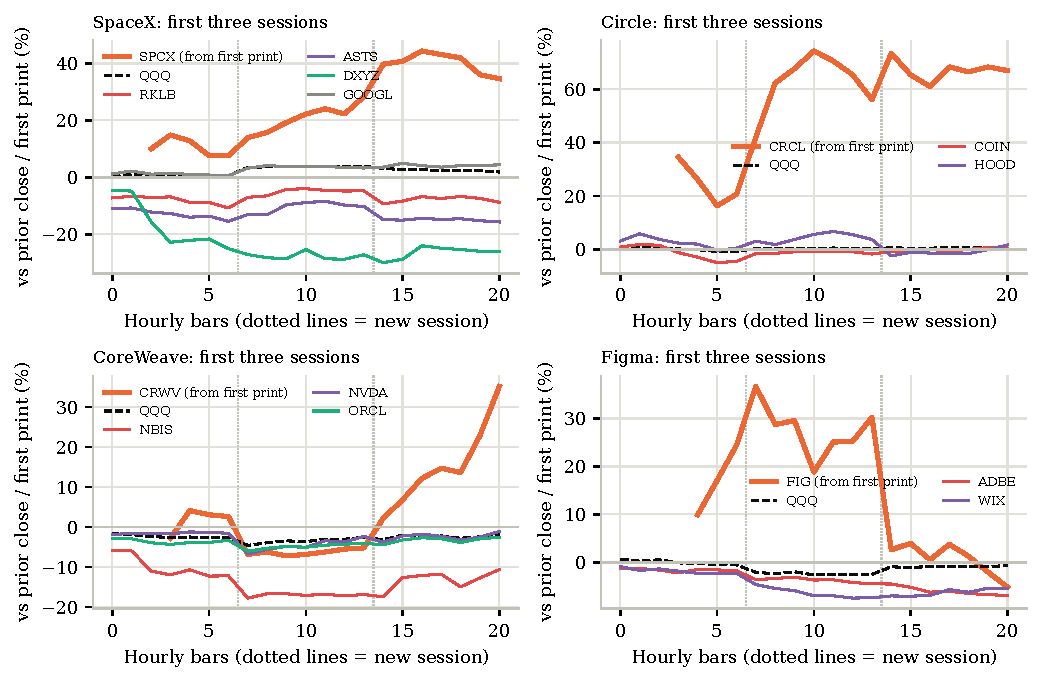
\includegraphics[width=\linewidth]{figures/g4_cases}
\caption{First three sessions, hourly. IPO (thick line) relative to its first print; peers, stakeholders and QQQ relative to the previous close. SpaceX's proxies gapped down and kept falling while SpaceX rose; Circle's peers sagged while Circle nearly tripled; CoreWeave and Figma show no transmission either way.}\label{fig:cases}
\end{figure}

\section{Anthropic: how the market is trading related stocks}
Table~\ref{tab:b7} and Figure~\ref{fig:ant} show where related stocks stand on 13 November, three trading days before pricing.

\begin{table}[!htbp]\centering\footnotesize
\caption{Stocks related to Anthropic into the IPO (to 13 November 2026)}\label{tab:b7}
\resizebox{\linewidth}{!}{
\begin{threeparttable}
\begin{tabular}{llrrrrrr}
\toprule
Ticker & Role & Beta & Since 30 Sep & Since S-1 (26 Oct) & Roadshow week & 20-day abnormal & Cohort pct \\
\midrule
NBIS & peer & 2.8 & $-$50.9 & $-$27.0 & $-$18.1 & $-$17.0 & 7 \\
CRWV & peer & 2.4 & $-$39.0 & $-$2.0 & +8.5 & +1.6 & 71 \\
NVDA & peer & 1.3 & $-$28.7 & $-$22.8 & $-$8.9 & $-$21.1 & 6 \\
AVGO & peer & 1.6 & $-$1.2 & +7.9 & +8.6 & +13.5 & 89 \\
ORCL & peer & 1.4 & $-$8.4 & $-$0.6 & +4.6 & +5.3 & 82 \\
PLTR & peer & 1.3 & $-$10.2 & $-$14.6 & $-$0.7 & $-$3.9 & 37 \\
MSFT & peer & 0.5 & +2.1 & $-$0.1 & $-$3.9 & +1.6 & 71 \\
AMZN & holder & 0.8 & +7.0 & +7.5 & $-$0.1 & +10.3 & 88 \\
GOOGL & holder & 0.8 & $-$14.0 & $-$7.6 & +2.6 & $-$10.0 & 17 \\
\midrule
SMH & index & 1.8 & $-$20.1 & $-$7.7 & $-$0.1 & $-$1.7 & -- \\
IGV & index & 0.8 & $-$5.0 & $-$8.5 & $-$0.3 & +0.2 & -- \\
ARKK & index & 1.5 & $-$15.8 & $-$8.5 & $-$5.1 & $-$1.8 & -- \\
QQQ & index & 1.0 & $-$8.1 & $-$3.5 & +0.1 & 0.0 & -- \\
\bottomrule
\end{tabular}
\begin{tablenotes}[flushleft]\footnotesize
\item \textit{Notes:} Raw returns except the 20-day abnormal return (vs QQQ market model). Roadshow week = 9 to 13 November. Cohort pct = percentile of the 20-day abnormal return within the 20-day pre-IPO abnormal returns of the cohort's 102 peer--IPO pairs. Holders = listed companies with a stake in Anthropic.
\end{tablenotes}
\end{threeparttable}
}
\end{table}


Three things stand out. First, AI infrastructure has de-rated hard since the end of September: Nebius $-51\%$, CoreWeave $-39\%$, Nvidia $-29\%$, the semiconductor ETF $-20\%$, against $-8\%$ for Nasdaq-100. Nebius's and Nvidia's 20-day abnormal returns rank in the bottom 7\% of what cohort peers did in the 20 days before their IPOs, where the cohort average is close to zero. Second, the two shareholders have diverged: Amazon is up 7\% (20-day abnormal $+10\%$, 88th percentile), Google down 14\%. Third, the roadshow week itself was mixed: CoreWeave, Broadcom and Oracle rose, Nebius and Nvidia fell.

The pattern resembles SpaceX more than the cohort average. SpaceX's proxies other than AST fell 14--22\% against QQQ in the 20 days before its IPO, then fell again on the day. Whether the AI sell-off is related to Anthropic at all cannot be established from prices: it coincides with doubts about AI capital spending and with a broad fall in speculative assets, which the companion paper measures as the lowest crowding reading of any IPO in the sample. What can be said is that the substitution trade, if there is one, has been running for six weeks, and that Anthropic is a better candidate for it than CoreWeave was. It is the first listed frontier-model company, and until now public investors could only reach it indirectly, through its compute suppliers and through Amazon and Google.

\begin{figure}[!htbp]\centering
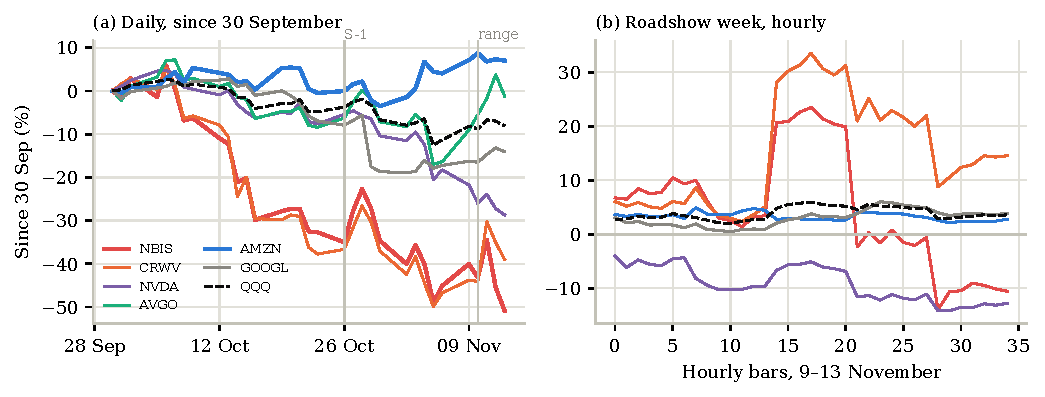
\includegraphics[width=\linewidth]{figures/g5_ant}
\caption{(a) Anthropic-related stocks since 30 September 2026; vertical lines at the public S-1 (26 October) and range setting (10 November). (b) Hourly, roadshow week, relative to the 6 November close.}\label{fig:ant}
\end{figure}

\section{Does Anthropic up mean Nebius up?}
Table~\ref{tab:b9} turns the cohort's betas into a mapping. If Anthropic trades 30\% above Nasdaq-100 on its first day, the daily co-movement coefficient implies a peer move of about $+2.6\%$ and the debut-week intraday beta about $+0.7\%$. Applied to a stock with Nebius's beta, that is noise. The mapping ignores substitution, which in the two closest precedents for a scarce-asset listing pushed peers the other way by more than the sympathy effect.

\begin{table}[!htbp]\centering\footnotesize
\caption{What the cohort's betas imply for peers if Anthropic moves}\label{tab:b9}

\begin{threeparttable}
\begin{tabular}{rrr}
\toprule
Anthropic move vs QQQ & Peers, daily beta (0.086) & Peers, intraday beta days 1--5 (0.024) \\
\midrule
$-$10 & $-$0.9 & $-$0.24 \\
+10 & +0.9 & +0.24 \\
+30 & +2.6 & +0.73 \\
+60 & +5.1 & +1.47 \\
\bottomrule
\end{tabular}
\begin{tablenotes}[flushleft]\footnotesize
\item \textit{Notes:} Mechanical mapping using the pooled coefficients of Tables~\ref{tab:b4} and~\ref{tab:b5}; it ignores the proxy unwind seen in SpaceX and Circle, which went the other way (Section~6).
\end{tablenotes}
\end{threeparttable}

\end{table}


The evidence therefore does not support trading AI peers as leveraged Anthropic beta on the day. Three trades are better supported:
\begin{enumerate}[leftmargin=1.4em]
\item \textbf{Own the IPO, not the proxy.} The return is in the allocation (companion paper); the proxies' best case is a small sympathy move and their worst case is the SpaceX-style unwind.
\item \textbf{If expressing a view through peers, do it after the debut week.} Co-movement builds over two to three months. A view on the theme is better expressed once Anthropic is seasoned and its correlation with the group has risen.
\item \textbf{Watch the 63-day co-fade.} IPO and peers fade together over a quarter ($\rho=0.46$). If Anthropic follows the hot-deal pattern and fades, AI peers are more likely to fade with it than to diverge.
\end{enumerate}

\section{Hypotheses for 19 November and after}
\begin{description}[leftmargin=1.2em,style=nextline]
\item[H1. No intraday beta.] During Anthropic's first session, the hourly correlation of Nebius, CoreWeave and Nvidia (excess of QQQ) with Anthropic will be below 0.2 and the beta below 0.05.
\item[H2. No sympathy on the day.] The AI peer basket's abnormal return on 19 November will be within $\pm2\%$ whatever the size of the pop; a pop above 30\% will not produce a peer move above $+3\%$.
\item[H3. Substitution, if any, shows up in the purest proxies.] If there is a proxy unwind, it will be in the highest-beta, most Anthropic-like listed exposures (Nebius, CoreWeave), from the first print to the close, and not in Amazon or Google.
\item[H4. Correlation builds.] Anthropic's daily correlation with the AI basket will be around 0.3 in its first month and nearer 0.5 after three months; its volatility will start at roughly twice the basket's.
\item[H5. The quarter.] Anthropic's and the AI basket's returns from 19 November to mid-February will have the same sign more often than not, and peers will not outperform QQQ over that window if Anthropic fades.
\end{description}

\section{Limitations}
Peer selection is judgemental, and a few comparables were delisted and are missing (CyberArk, Eventbrite, Redfin, Owens \& Minor, eXp). Hourly data cover 14 IPOs, and only two of them are scarce-asset listings, so the substitution result rests on two cases plus the mechanism. Overlapping peers and clustered listing dates (2021, September 2025) reduce the effective sample. Market-model abnormal returns for very high-beta stocks are noisy, as the wide placebo distribution shows. For Anthropic, the price moves in Table~\ref{tab:b7} cannot be attributed to the IPO: they coincide with a broad de-rating of AI and speculative assets.

\section{Conclusion}
Large IPOs do not move their peers on the day or intraday. In the debut week the new stock trades on its own flows; its correlation with its peers, and the peers' response to it, build only as it seasons. The exception is the listing of a scarce asset, where the listed proxies lose their premium as the real thing becomes available. Anthropic is closer to that case than any previous AI listing, and its nearest proxies have already fallen 30--50\% since September. For the debut, the honest answer to ``Anthropic up, Nebius up?'' is: not by much, and quite possibly the other way.

\bibliographystyle{plainnat}
\bibliography{refs}

\appendix
\section{Peer map}\label{app:map}
{\scriptsize
\begin{longtable}{lll}
\toprule IPO & Comparables & Listed stakeholders \\ \midrule \endhead
Snowflake (SNOW) & MDB, DDOG, NET & -- \\
Unity (U) & EA, TTWO & -- \\
Arm (ARM) & NVDA, AMD, QCOM, AVGO & -- \\
Klaviyo (KVYO) & HUBS, BRZE & SHOP \\
Astera Labs (ALAB) & AVGO, MRVL, CRDO & -- \\
CoreWeave (CRWV) & NBIS, ORCL, SMCI & NVDA \\
Figma (FIG) & ADBE, WIX & -- \\
Duolingo (DUOL) & CHGG, COUR & -- \\
Rubrik (RBRK) & CRWD, PANW, NTNX & -- \\
Netskope (NTSK) & ZS, CRWD, PANW, NET & -- \\
SailPoint (SAIL) & OKTA, CYBR, CRWD & -- \\
Toast (TOST) & XYZ, FOUR, PAR & -- \\
Airbnb (ABNB) & BKNG, EXPE & -- \\
DoorDash (DASH) & UBER, LYFT & -- \\
Coupang (CPNG) & AMZN, MELI, SE & -- \\
Instacart (CART) & DASH, UBER, KR & -- \\
Reddit (RDDT) & META, PINS, SNAP & -- \\
Bumble (BMBL) & MTCH & -- \\
StubHub (STUB) & EB, LYV, SEAT & -- \\
Compass (COMP) & Z, RDFN, EXPI & -- \\
Robinhood (HOOD) & SCHW, IBKR, COIN & -- \\
Affirm (AFRM) & PYPL, XYZ, UPST & -- \\
Circle (CRCL) & HOOD & COIN \\
Chime (CHYM) & SOFI, NU, DAVE & -- \\
Klarna (KLAR) & AFRM, PYPL, SEZL & -- \\
eToro (ETOR) & HOOD, COIN, IBKR & -- \\
Figure (FIGR) & SOFI, UPST, COIN & -- \\
Gemini (GEMI) & COIN, HOOD, CRCL & -- \\
Oscar Health (OSCR) & UNH, HUM, CLOV & -- \\
Medline (MDLN) & OMI, CAH, MCK & -- \\
Tempus AI (TEM) & GH, NTRA & -- \\
Waystar (WAY) & EVH, PHR & -- \\
Hinge Health (HNGE) & TDOC, HIMS & -- \\
Cava (CAVA) & CMG, SG, WING & -- \\
Birkenstock (BIRK) & DECK, CROX, NKE & -- \\
Viking (VIK) & RCL, CCL, NCLH & -- \\
Ibotta (IBTA) & CART, TTD & -- \\
Rivian (RIVN) & TSLA, LCID & AMZN, F \\
Lineage (LINE) & COLD, PLD & -- \\
StandardAero (SARO) & HEI, TDG, FTAI & -- \\
Nextracker (NXT) & ARRY, SHLS, FSLR & -- \\
Venture Global (VG) & LNG, NFE & -- \\
SpaceX (SPCX) & RKLB, ASTS & GOOGL, DXYZ \\
Anthropic (ANT) & NBIS, CRWV, ORCL, NVDA, AVGO, PLTR, MSFT & AMZN, GOOGL \\
\bottomrule
\end{longtable}}


\section{Data and replication}
\texttt{beta\_collect.py} downloads daily and hourly bars and writes the peer map; \texttt{beta\_trade.py} computes the event study, placebo, co-movement, hourly tests and the Anthropic snapshot (\texttt{data/beta.json}); \texttt{paper\_beta/make\_paper4.py} builds the tables and figures. Signals and IPO outcomes come from \texttt{signals.py}.
\end{document}
